\documentclass[11pt, letterpaper]{article}
\usepackage[utf8]{inputenc}
\usepackage[margin=1in]{geometry}
\usepackage{graphicx}
\usepackage{hyperref}
\usepackage{xcolor}
\usepackage[justification=centering]{caption}

% \hypersetup{
%     colorlinks,
%     linkcolor={red!50!black},
%     citecolor={blue!50!black},
%     urlcolor={blue!80!black}
% }

% geometry: for page margins
% graphicx: for inserting images
% hyperref: for adding hyperlinks to Figure references

% location for images
\graphicspath{ {./figures/} }

\setlength{\parskip}{1em}

\title{\textbf{Human Pose Estimation: Progress Report}}
\author{Robert Lee, Julian Rocha, Wanze Zhang, Nicole Peverley, Rafay Chaudhry, Corey Koelewyn}
\date{\today}

\begin{document}

\maketitle

\section{The Problem}

Human pose estimation (HPE) is the problem domain of identifying body keypoints to construct a body model. Many existing systems accept images as input, with some implementations accepting formats such as point cloud and videos. The application of HPE is widespread and benefits many industries. In particular, HPE is used for animation in both the film and gaming industries. A more sinister application of HPE can be used for identification of individuals over multiple frames (i.e., videos). Another subset of HPE is hand pose estimation which can be used to translate sign language. HPE is a difficult problem domain due to a number of challenges. These include variability in human appearance and physique, environment lighting and weather, occlusions from other objects, self-occlusions from overlapping joints, complexity of movements of the human skeleton, and the inherent loss of information with a 2D image input \cite{Sigal2014}. This largely unsolved problem enables us to explore many novel and creative approaches, enriching our learning experience. We are excited to explore these applications, but we decided to limit our scope to a general version of the problem so we could reference the abundance of research available.

There are many variations of HPE systems, which can be roughly categorized into 2D vs 3D, single-person vs multi-person, and different body models. Our group plans to focus on single-frame monocular RGB images containing a single individual rather than a photo with multiple individuals. We believe it will be more feasible to train a deep neural network (NN) with one individual based upon the research papers available and in the given timeframe. Given success with single individuals, we may explore multi-person HPE. Current state-of-the-art techniques for 2D single-person HPE can be categorized into two categories: regression on absolute joint position, or heat maps on approximate joint location. Regression-based techniques were generally used in older projects, whereas heat maps are a popular technique currently. Based on our research, we believe that the newer method (heatmaps) will yield more accurate results. Accordingly, we are opting to use a heat map-based approach within our network.

\begin{figure}
    \centering
    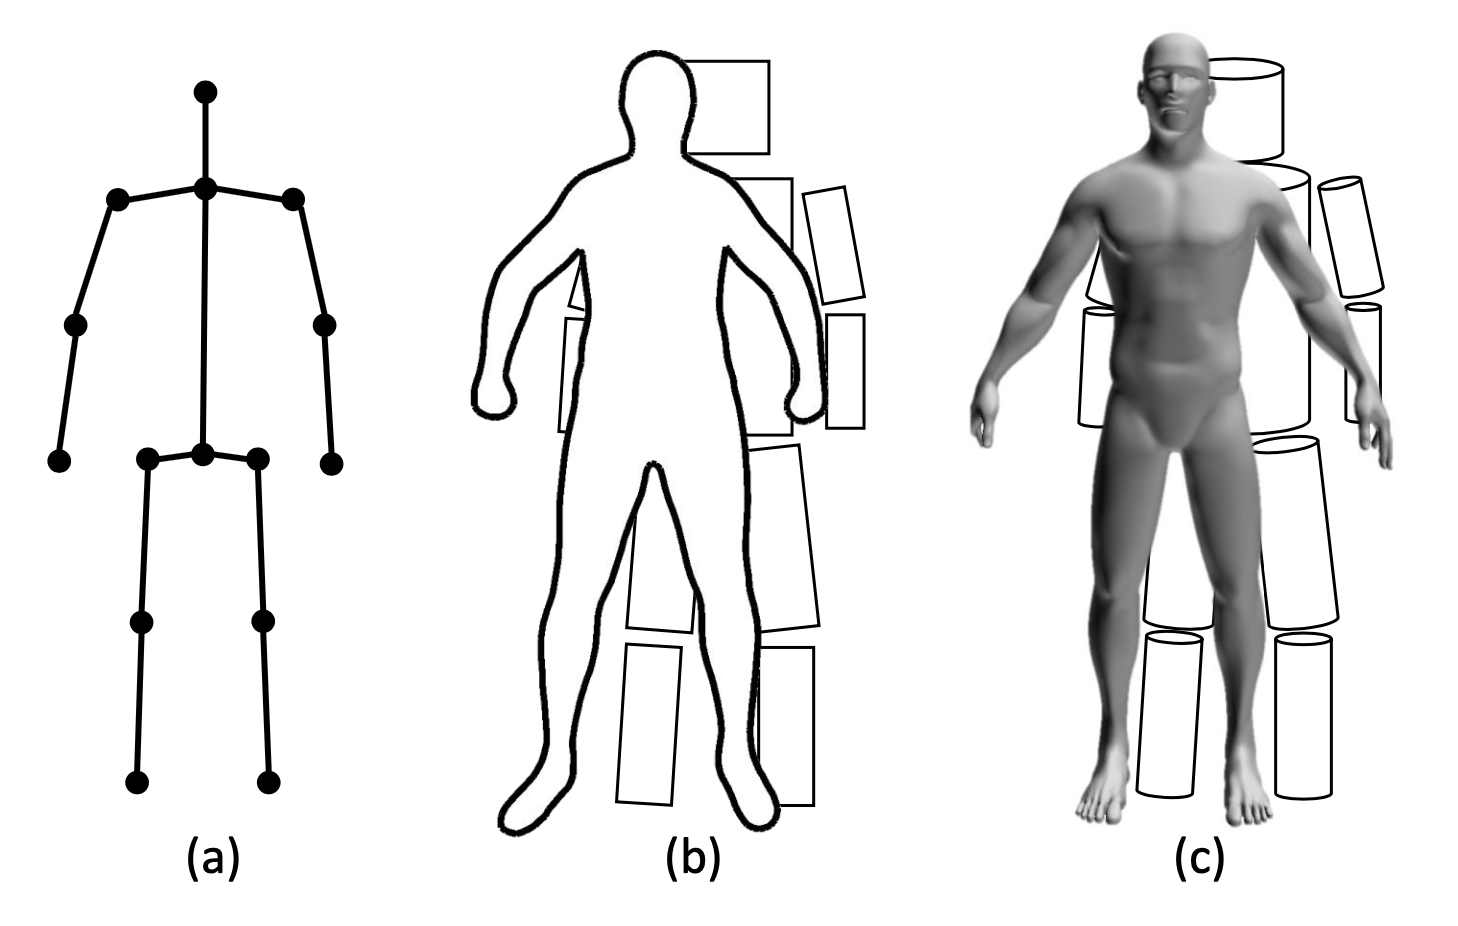
\includegraphics[width=0.75\textwidth]{body_models.png}
    \caption{Common body models: (a) skeleton-based, (b) contour-based, (c) volume-based \cite{Chen_2020}}
    \label{fig:body_model}
\end{figure}

There are three different types of models used with full body HPE: kinematic, contour, and volumetric, as shown in Fig. \ref{fig:body_model} \cite{Chen_2020}. A kinematic model consists of points on each human joint connected by straight lines, similar to a stick-figure skeleton. The contour model consists of 2D squares and rectangles that represent the body, and the volumetric model represents the body with 3D cylinders. Further high-fidelity models implement meshes that capture more details of the human pose. The kinematic model is the simplest model to perform loss metric computations, and thus is preferred by our group as a scope-limiting decision. Using a basic kinematic model will simplify the problem space and encourage us to focus on tangible results that can be used in real life applications. Our goal is to estimate a kinematic model for the individual in each picture.

While there were many existing HPE datasets, very few perfectly matched our chosen requirements for the project. Any available datasets would need to be cleaned and processed. Many datasets contained assorted images that used different types of models for the pose estimation or consisted of multiple people in each image. Our primary choice is the COCO dataset \cite{coco_data}. This dataset consists of 330 K images, of which 200 K are labelled. There are pre-sorted subsets of this dataset specific for HPE competitions: COCO16 and COCO17. These contain 147 K images labelled with bounding boxes, joint locations, and human body masks. We may explore using DensePose \cite{densepose}, which is a highly detailed manually annotated subset of the COCO dataset. Currently, the DensePose dataset seems unlikely to work for our requirements due to the pose estimation model we have chosen. If other preferred datasets are not available, we plan to use the MPII dataset, which consists of 41 K labelled images split into 29 K train and 12 K test \cite{mpii}. If time permits, we may validate our model’s performance on this secondary dataset. 


\section{Goals}


\section{Plans and Progress To Date}



\section{Task Breakdown}



\section{Initial Results}



% TODO delete below

% To add a figure, use the following:

% \begin{figure}[h]
%     \centering
%     \includegraphics[width=0.5\textwidth]{FIGURE_NAME_HERE}
%     \caption{a nice plot}
%     \label{fig:fig1}
% \end{figure}

% To reference a figure, use the following:
% \ref{fig:fig1}

% To cite, use the following:
% \cite{NAME_HERE}

% Lorem ipsum dolor sit amet Fig. , consectetur adipiscing elit. Proin rhoncus mollis libero, non auctor risus feugiat ac. Quisque nec urna eu diam placerat gravida.\cite{Yan2013} Etiam rhoncus \cite{overleaf} $E=mc^2$.

% \begin{equation}
%     E=mc^2
% \end{equation}

\newpage

\bibliographystyle{IEEEtran}
\bibliography{references}

\end{document}